\chapter{ODE Data Representation}
In the Drasil framework, there is a single data structure containing all the information for all products, and we call it \verb|System Information|. The giant \verb|System Information| collects a multitude of pieces of information; whenever we need it, we extract the information from the \verb|System Information|. We store the ODE information in \verb|System Information|. 

A ODE could existed in various forms and some forms was designed for specific purposes. For example, we can transform a higher-order ODE to its equivalent system of first-order ODE. Then, we can solve the system of ODE numerically. In previous research, We stored the ODE information in a data structure that cannot be re-used for other purposes. We have to re-write the ODE in a specific form to satisfy a new goal each time. It starts propagate duplication and we easily lose traceability. Therefore, the Drasil team is exploring new way to store ODEs in a new data structure, and the new structure would allow ODEs be isomorphic, which means we can map one ODE form to others. 

By capturing the essential information of ODEs, we can flexibly transform it in others forms that might similarly appear. On one hand, the transformation might result in losing information. For example, we can display ODE in a textual form in SRS (software requirements specification). Once we completed transformation for displaying purpose, the textual form ODE has less information than the original ODE. On the other hand, we made transformation for a specific purpose, such as generating ODE in code. Furthermore, capturing ODEs information in a flexible data structure only requires Drasil users write ODEs once.

In this chapter, we will first introduce how we re-write ODE for a different purpose. Then, we will introduce a new data structure for storing ODE information. We will talk about details on how the new data structure captures ODE information, how to use the new data structure, and how the new data structure interacts with Drasil Printer.

\section{Explicit Equation}
Before we conduct this research, the Drasil framework can generate software that provides numerical solutions for a first-order ODE by explicitly rewriting the ODE equation. We re-write the original ODE in a form which the Drasil Code Generator can utilize. The Drasil Code Generator retrieve ODE information from the new ODE equation, and generate a program that can produce numerical solutions. Here is the example how we solve the \href{https://jacquescarette.github.io/Drasil/examples/nopcm/SRS/srs/NoPCM_SRS.html#Sec:IMs}{NoPCM case study}. The Equation~\ref{eq_nopcmorginal} was defined in \verb|Instance Model|. The model describes the energy balance of water, and we can find the temperature of the water base on it.

\begin{equation} \label{eq_nopcmorginal}
	T_{w}'(t) +  \frac {T_{w}(t)}{\tau_{w}} = \frac{T_{c}}{\tau_{w}}
\end{equation}
\myequations{NoPCM Equation}

The $T_w(t)$ is a function of the independent variable, in this case time. The $T_w$ is the temperature of water ($ ^\circ C $). The $T_w'(t)$ is the first directive of the function $T_w(t)$ respect time. The $T_c$ is the temperature of the heating coil (°C), and the $\tau_w$ is the ODE parameter for water related to decay time (s). Isolating for $T_w'(t)$, we obtain the following Equation~\ref{eq_nopcmderive}.
\begin{equation} \label{eq_nopcmderive}
	T_{w}'(t) = \frac{T_{c} - T_{w}(t)}{\tau_{w}}
\end{equation}

\begin{listing}[ht]
\begin{haskell1}
-- Pseudocode
T_w'(t) = reciprocal τ_w * (T_c - T_w(t))
\end{haskell1}
\captionof{listing}{NoPCM equation for SRS}
\label{code_expliciteqsrs}
\end{listing}

Based on Equation~\ref{eq_nopcmderive}, we can write it into a text-based form. A form that text be literarily written down. It does not contain rich data. Code~\ref{code_expliciteqsrs} shows how to textually encode Equation~\ref{eq_nopcmderive} in Drasil. We can use the information of Code~\ref{code_expliciteqsrs} for displaying purpose, such as displaying ODE equation in SRS, because we wrote them down literarily. However, we cannot reuse it for other purpose such as creating a program which solve the ODE numerically. Therefore, we re-write the Code~\ref{code_expliciteqsrs} to other form for solving purpose. Brooks's thesis~\citep{brooks} documented how the Drasil framework solves Equation~\ref{eq_nopcmderive} with manually created \href{https://jacquescarette.github.io/Drasil/docs/drasil-code-0.1.9.0/Language-Drasil-Code.html#t:ODEInfo}{ODEInfo}. The \verb|ODEInfo| is a \verb|data type| that extract useful information from the original ODE (Equation~\ref{eq_nopcmderive}). Drasil Code Generator can utilize \verb|ODEInfo| to generate a program that solve the original ODE numerically. 
\begin{listing}[ht]
\begin{haskell1}
-- Pseudocode
reciprocal τ_w * (T_c - T_w[0])
\end{haskell1}
\captionof{listing}{NoPCM equation for the Drasil Code Generator}
\label{code_expliciteq}
\end{listing}
Code~\ref{code_expliciteq} shows how to rewriting the original ODE for solving purpose. We can not directly transform Code~\ref{code_expliciteqsrs} to Code~\ref{code_expliciteq}, there is a gap between two ODE expressions.

Despite the gap between Code~\ref{code_expliciteqsrs} and Code~\ref{code_expliciteq}, we can manually close it by re-writing the ODE. Rewriting the ODE in other form produce duplication because both Code~\ref{code_expliciteqsrs} and Code~\ref{code_expliciteq} describe the same ODE. The Code~\ref{code_expliciteqsrs} lacks the necessary structure to allow transformation. Therefore, the Drasil team decided to make an new data structure to store the ODE information, so the ODE information can be reused for different purposes.

% The user will first encode the ODE equation in the general data pool. Whenever we need it, we retrieve the ODE equation from it. However, there is a gap between the original equation and external libraries (Chapter~\ref{cha_extlib}). The external libraries can not understand the original ODE equation from the general data pool. Therefore, the Drasil team manually transforms the original ODE equation into another form (\verb|ODEInfo|), which external libraries can use to produce a numerical solution.

% Here is an example of how we manually close the gap between the text-based ODE and external libraries. In Code~\ref{code_expliciteqsrs}, we encode Equation~\ref{eq_nopcmderive} and put it into the general data pool. During printing the SRS, we retrieve the text-based ODE and print it. The Drasil printer is capable of displaying encoded ODE in text. However, external libraries require a specific format for the ODE and can not utilize the original ODE. Therefore, we manually create Code \ref{code_expliciteq} so external libraries can solve the ODE. They both describe the same ODE, but we write it twice in the Drasil framework. Therefore, there is an information duplication. We can transform from Code~\ref{code_expliciteqsrs} to Code~\ref{code_expliciteq} with human interference. However, without human interference, we can not complete the transformation because Code~\ref{code_expliciteqsrs} lacks the necessary structure. To reduce the information duplication, 

\section{Matrix Form Structure}
In general, an equation contains a left-hand expression, a right-hand expression, and an equal sign. The left-hand and right-hand expressions connect by an equal sign. A linear ODE also has its left-hand and right-hand sides. Each side has its unique shape. We can write a linear ODE in the shape of
\begin{equation} \label{eq_matrixform}
	\boldsymbol{Ax} = \boldsymbol{b}
\end{equation}
\myequations{Matrix Form}

On the left-hand side, \textbf{A} is an m $\times$ n matrix, and \textbf{x} is an n-vector. On the right-hand side, \textbf{b} is an m-vector. The \textbf{A} is commonly known as the coefficient matrix, \textbf{x} is the unknown vector, and \textbf{b} is the constant vector. The equation~\ref{eq_matrixform} can represent not only a single linear ODE, but also represent a linear system of ODE. A linear system of ODE is a finite set of linear differential equations. In this research, we only have case studies for single ODEs, and all examples will demonstrate on single ODEs. The new data structure we proposed is capable to store information for a system of ODE, but its related functions only support for case studies that has single ODEs. Here is an ODE example from \href{https://jacquescarette.github.io/Drasil/examples/pdcontroller/SRS/srs/PDController_SRS.html#Sec:IMs}{PDContoller case study}.
\begin{equation} \label{eq_odeexmaple}
	y''(t) + (1 + K_d) \cdot y'(t) + (20 + K_p) \cdot y(t) = r_t \cdot K_p
\end{equation}
\myequations{PDContoller Equation}

In Example~\ref{eq_odeexmaple}, there is only one dependent variable $y$. The dependent variable $y$ is depend on independent variable t, in this case time. We use $y$(t) to represent a function of time. The $y'$(t) is the first derivative of $y$(t). The $y''$(t) is the second derivative of $y$(t). The $y$ is the process variable, and the $y'(t)$ is the rate of change of $y(t)$. The $y''(t)$ is the rate of change of the rate of change of $y(t)$. The $K_d$ , $K_p$, and $r_t$ are constant variables. The $K_d$ is Derivative Gain, $K_p$ is Proportional Gain, and $r_t$ is Set-Point. We can write this equation in a matrix form as follows.

\begin{equation} \label{eq_matrixformexmaple}
	\begin{bmatrix}
		1, & 1 + K_{d}, & 20 + K_{p}
	\end{bmatrix}
	\cdot
	\begin{bmatrix}
		y''(t)  \\
		y'(t)   \\
		y(t)  
	\end{bmatrix}
	=
	\begin{bmatrix}
		r_{t} \cdot K_{p} 
	\end{bmatrix}
\end{equation}
\myequations{PDContoller Equation in Matrix Form}

The relationship between the matrix form~\ref{eq_matrixform} and the example~\ref{eq_matrixformexmaple} is not hard to find. Firstly, the coefficient matrix \textbf{A} is a 1 $\times$ 3 matrix that consists of $1$, $1 + K_d$, ane $20 + K_p$. Secondly, the unknown vector \textbf{x} is a 3 $\times$ 1 vector with $y''$, $y'$, and $y$. Last, the constant vector \textbf{b} is a 1 $\times$ 1 vector with $r_t \cdot K_p$. The matrix form~\ref{eq_matrixform} very well captures all the knowledge we need to present an ODE. But, how a matrix form looks like in a nth-order linear ODE? Based on Paul's Online Notes~\citep{paullinearode}, we can write all linear ODEs in the shape of

\begin{equation} \label{eq_linearDE}
	a_n(t) \cdot y^n(t) + a_{n-1}(t) \cdot y^{n-1}(t) + \dots + a_1(t) \cdot y'(t) + a_0(t) \cdot y(t) = h(t)
\end{equation}
\myequations{Linear Higher-Order ODE}

The coefficient $a_0(t), \dots, a_n(t)$ and $g(t)$ can be constant or non-constant functions, in our case they are constant functions. We also can write Equation~\ref{eq_linearDE} in a matrix form. 
\begin{equation} \label{eq_matrixnthorder}
	\begin{bmatrix}
		a_n(t), & a_{n-1}, \dots, & a_0(t)
	\end{bmatrix}
	\cdot
	\begin{bmatrix}
		y^{n}(t) \\
		y^{n-1}(t) \\
		\dots \\
		y(t)  
	\end{bmatrix}
	=
	\begin{bmatrix}
		h(t)
	\end{bmatrix}
\end{equation}
\myequations{Linear Higher-Order ODE in Matrix Form}

This is the methodology used for linear ODEs, and it contains all necessary information for understanding the linear ODE. Therefore, we create a data structure which contain the matrix information of the ODE. It is an advanced structural ODE information \verb|data type|, called \verb|DifferentialModel| to capture knowledge of linear ODEs.

The \verb|DifferentialModel| is the type, it takes one value. The \verb|SystemOfLinearODEs| is a value with a record that is used to describe a structural content of system of linear ODEs with six necessary fields. Here is the representing code for \verb|DifferentialModel|.
\begin{haskell1}
data DifferentialModel = SystemOfLinearODEs {
	_indepVar :: UnitalChunk,
	_depVar :: ConstrConcept,
	_coefficients :: [[Expr]],
	_unknowns :: [Unknown],
	_dmConstants :: [Expr],
	_dmconc :: ConceptChunk
}
\end{haskell1}

Previous to this research, \href{https://jacquescarette.github.io/Drasil/docs/full/drasil-lang-0.1.60.0/Language-Drasil-Chunk-Unital.html#t:UnitalChunk}{UnitalChunk}, \href{https://jacquescarette.github.io/Drasil/docs/full/drasil-lang-0.1.60.0/Language-Drasil-Chunk-Constrained.html#t:ConstrConcept}{ConstrConcept}, \href{https://jacquescarette.github.io/Drasil/docs/full/drasil-lang-0.1.60.0/Language-Drasil-Expr-Lang.html#t:Expr}{Expr}, and \href{https://jacquescarette.github.io/Drasil/docs/full/drasil-lang-0.1.60.0/Language-Drasil-Chunk-Concept-Core.html#t:ConceptChunk}{ConceptChunk} already existed in Drasil. We created an \verb|Unknown| type for this experiment. Their semantics will show up in Table~\ref{tab_demodeltype}
\begin{table}[ht]
	\begin{tabular}{ p{0.2\textwidth} p{0.7\textwidth} }
		\textbf{Type} & \textbf{Semantics} \\
		\toprule
		\verb|UnitalChunk| & concepts with quantities that must have a unit definition.\\
		\verb|ConstrConcept| & conceptual symbolic quantities with Constraints and maybe a reasonable value.\\
		\verb|Expr| & a type encode mathematical expression. \\
		\verb|ConceptChunk| & a concept that contains an idea, a definition, and an associated domain of knowledge\\
        \verb|Unknown|& synonym of Integer\\
		\bottomrule	
	\end{tabular}	
	\caption{Type use in DifferentialModel}	
	\label{tab_demodeltype}
\end{table}

The \verb|_indepVar| represents the independent variable, and it is often time. The \verb|_depVar| represents the dependent variable. Combing \verb|_depVar| and \verb|_indepVar|, it represents a function produce dependent variables over time. The \verb|_coefficients| is a list of lists \verb|Expr|, and it represents the coefficient matrix \textbf{A}. The \verb|_unknowns| is a list of \verb|Unknown|, and \verb|Unknown| is synonym of integers.
The \verb|_unknowns| represent a list of numbers of derivatives of the function. Combining \verb|_depVar|, \verb|_indepVar| and \verb|_unknowns|, they can represent the unknown vector \textbf{x}. The \verb|_dmConstants| is a list of \verb|Expr|, and it represents the constant vector \textbf{b}. Last, the \verb|_dmconc| contains metadata of this model. To represent example~\ref{eq_odeexmaple} in \verb|DifferentialModel|, \verb|_indepVar| is time, \verb|_depVar| is $y$, \verb|_coefficients| is the 1 $\times$ 3 matrix, \verb|_unknowns| is the 3 $\times$ 1 vector, \verb|_dmConstants| is the 1 $\times$ 1 vector, and \verb|_dmconc| is \verb|ConceptChunk| that describes what this model is. Code~\ref{code_interaldata} shows the internal data representation of the example~\ref{eq_odeexmaple} in \verb|DifferentialModel|.

\begin{listing}[ht]
\begin{haskell1}
_indepVar = time
_depVar = y
_coefficients = [[1, 1 + K_d, 20 + K_p]]
_unknowns = [2, 1, 0]
_dmConstants = [r_t * K_p]
_dmconc = ... -- Drasil definition for chuck concept
\end{haskell1}
\captionof{listing}{Internal Data Representation for Example~\ref{eq_odeexmaple}}
\label{code_interaldata}
\end{listing}

Currently, the \verb|DifferentialModel| only captures the knowledge of linear ODEs with one dependent variable, and it is a special case of the family of linear ODEs. Studying this special case will help the Drasil team better understand how to capture the knowledge of all ODEs and eventually lead to solving a system of linear ODE with multiple dependent variables. On top of that, there is one assumption: the \verb|_coefficients| can only be functions of independent variable \verb|_indepVar|, often time. In other word, the \verb|_coefficients| does not depend on the dependent variable \verb|_depVar|.

\section{Input Language}
\label{sec_input}
There are many reasons why we want to provide an input language for users to input ODE equations. One major reason is that it could be over complicated for users to input a single ODE in a matrix form. While inputting a single ODE, one obvious way is directly passing value to each record via constructors of \verb|DifferentialModel|. The Code~\ref{code_interaldata} shows how to encode Example~\ref{eq_odeexmaple} in the \verb|DifferentialModel|. However, it would be not so elegant to set a single ODE in the example, because users have to extracts the coefficient matrix \textbf{A}, unknown vector \textbf{x} and constant vector \textbf{b} from the original equation manually. Once the coefficient matrix, unknown vector and constant vector is ready, we can set value into \verb|_depVar|, \verb|_coefficients|, \verb|_unknowns|, and \verb|_dmConstants| accordingly. This process is ideal when the ODE is a system of ODE, and it would be over-complicated for user to do extraction for a single ODE. Therefore, we decided create a helper function to ease this issue. On top of that, the Drasil printer will print a single ODE in SRS with a more familiar ``one line equation'' form. Another advantage of having an helper function to input an ODE is that it can reduce human error and make sure the equation is well-formed. We call this helper function input language, and what will this input language looks like? 

The input language is inspired by how a linear nth-order ODE looks like. Based on Paul's Online Notes~\citep{paullinearode}, we can write all linear ODEs in the shape of Equation~\ref{eq_linearDE}. On the left-hand side of Equation~\ref{eq_linearDE}, the expression is a collection of terms. Each term consists of a coefficient function and a derivative of the function y(t). With ideas of term, coefficient, and derivative, we create new data types to mimic the mathematical expression of a linear ODE. The following is the detail of the code for new data types and operators.

\begin{haskell1}
type Unknown = Integer
data Term = T{
	_coeff :: Expr,
	_unk :: Unknown
}
type LHS = [Term]

($^^) :: ConstrConcept -> Integer -> Unknown
($^^) _ unk' = unk'

($*) :: Expr -> Unknown -> Term
($*) = T

($+) :: [Term] -> Term -> LHS
($+) xs x  = xs ++ [x]
\end{haskell1}

For new types, the \verb|LHS|, the short name for the left-hand side, is a list of \verb|Term|. This corresponds to the left hand side is a collection of terms. Each \verb|Term| has an \verb|Expr| and \verb|Unknown|. This corresponds to a term consists of a coefficient and a derivative of the function. Although \verb|_unk| is an integer, combining \verb|_unk|, \verb|_depVar| and \verb|_indepVar| we can get the derivative of the function. For new operators, they are inspired by the linear equation~\ref{eq_linearDE}. The \verb|$^^| operator take a variable and a integer, and it represents the derivative of the function. For instance, in example~\ref{eq_odeexmaple}, we can write $y(t)$\^{}\^{}2 to represent $y''(t)$. One thing we want to notice here is that we store $y(t)$ in \verb|_depVar| and \verb|_indepVar|. The operator \verb|$^^| will ignore the first parameter, and store the second parameter in \verb|_unknowns|. The reason to positioning a dummy variable before \verb|$^^| is becasue this will maintain the whole input structure as close as a linear ODE. The \verb|$*| operator creates a term by combining a coefficient matrix and a derivative function. For instance, in example~\ref{eq_odeexmaple}, we can write $(1 + K_d) \$* (y$ \$\^{}\^{}1) to represent $(1 + K_d) \cdot y'(t)$. Last, the \verb|$+| operator will append all terms into a list. Let's write pseudo code (Code \ref{code_exinputl}) for the example matrix form~\ref{eq_odeexmaple} in the newly introduced input language. The full detail of the input language for the PDController example will show up in ~\ref{const_de}.

\begin{listing}[ht]
\begin{haskell1}
-- in Example \ref{eq_odeexmaple}: y\_t'' + (1 + K\_d)y\_t' + (20 + K\_p)y\_t = r\_t K\_p
-- left hand side = y\_t'' + (1 + K\_d)y\_t' + (20 + K\_p)y\_t 
-- right hand side = r\_t K\_p

lhs = [1 $* (y $^^ 2)]
	$+ (1 + K_d) $* (y $^^ 1)
	$+ (20 + K_p) $* (y $^^ 0)
rhs = r_t * K_p
\end{haskell1}
\captionof{listing}{Input language for the example~\ref{eq_odeexmaple}}
\label{code_exinputl}
\end{listing}

\section{Two Constructors}
There are many way to create the \verb|DifferentialModel|. One most obvious way is to set each field directly by passing values in the constructor and \href{https://jacquescarette.github.io/Drasil/docs/full/drasil-lang-0.1.60.0/Language-Drasil-Chunk-DifferentialModel.html#t:makeASystemDE}{makeASystemDE} constructor serve as this role. We also designed another constructor, \href{https://jacquescarette.github.io/Drasil/docs/full/drasil-lang-0.1.60.0/Language-Drasil-Chunk-DifferentialModel.html#t:makeASingleDE}{makeASingleDE}, for users who want to use input language to create a \verb|DifferentialModel|.

For \verb|makeASystemDE| constructor, a user can set the coefficient matrix, unknown vector, and constant vector by explicitly giving \verb|[[Expr]]|, \verb|[Unknown]|, and \verb|[Expr]|. There will be several guards to check whether inputs are well-formed.

1. The coefficient matrix and constant vector dimension need to match. The \verb|_coefficients| is an m $\times$ n matrix, and \verb|_dmConstants| is an m vector. This guard makes sure they have the same m dimension. If the dimensions do not match, Drasil framework will throw an error: ``Length of coefficients matrix should equal to the length of the constant vector''. It means \verb|_coefficients| and \verb|_dmConstants| has different m dimension and violating mathematical rules.

2. The dimension of each row in the coefficient matrix and unknown vector need to match. The \verb|_coefficients| use a list of lists to represent an m $\times$ n matrix. It means each list in \verb|_coefficients| will have the same length n, and \verb|_unknowns| is an n-vector. Therefore, the length of each row in the \verb|_coefficients| should equal the length of \verb|_unknowns|. If an error says, ``The length of each row vector in coefficients need to equal to the length of unknowns vector.'', it means \verb|_coefficients| and \verb|_unknowns| violate mathematical rules.

3. The order of the unknown vector needs to be descending due to design decisions. We have no control over what users will give to us, and there are infinite ways to represent a linear equation in the matrix form~\ref{eq_matrixform}. We strictly ask users to input the unknown vector descending, so we can maintain the shape of a normal form of linear ODE~\ref{eq_linearDE}. This design decision will simplify the implementation for solving a linear ODE numerically in Chapter 3. If an error says, ``The order of giving unknowns needs to be descending.'', it means the order of unknown vector is not descending.

Code~\ref{code_scexmatrix} is pseudocode shows how to directly set the example~\ref{eq_odeexmaple}'s coefficient matrix, unknown vector, and constant vector. This example is made for \href{https://jacquescarette.github.io/Drasil/examples/pdcontroller/SRS/srs/PDController_SRS.html}{PDContoller} case study.

\begin{listing}[ht]
\begin{haskell1}
imPDRC :: DifferentialModel
imPDRC = makeASystemDE
	time
	opProcessVariable
	coeffs = [[1, 1 + K_d, 20 + K_p]]
	unknowns = [2, 1, 0]
	constants = [r_t * K_p]
	"imPDRC"
	(nounPhraseSP "Computation of the Process Variable as a function of time")
	EmptyS
\end{haskell1}
\captionof{listing}{Explicitly set values for the example~\ref{eq_odeexmaple} in DifferentialModel}
\label{code_scexmatrix}
\end{listing}

The second constructor is called \verb|makeASingleDE|. This constructor uses the input language to simplify the input of a single ODE. In \verb|makeASingleDE|, we create the coefficient matrix, unknown vector, and constant vector based on restricted inputs. Contrasting to the \verb|makeASystemDE|, users have to input ODE by using input language we designed. In the backend, the \verb|DifferentialModel| will extract useful information from the input ODE, and generate the coefficient matrix and unknown vector. The constructor first creates a descending unknown vector base on the highest number of its derivatives. To take the code~\ref{code_exinputl} as an example, the highest order of its derivative on the left-hand side (\verb|lhs|) is 2, so we will generate the unknown vector $[2, 1, 0]$. Then, based on generated unknown vector, we will search the correspond coefficient from the input ODE, and form a matrix. The main advantage of this design decision is that we rely on the input language to provide the ODE in a correct format. While we allowing users directly set values for \verb|DifferentialModel|, we have no guarantee the format of input is correct. With help from the input language, users can check syntax errors. The pseudocode~\ref{code_exinputl} shows how to use the input language to set Example~\ref{eq_odeexmaple} in a matrix form. The full detail of how to use the input language set the coefficient matrix, unknown vector, and constant vector for the \href{https://jacquescarette.github.io/Drasil/examples/pdcontroller/SRS/srs/PDController_SRS.html}{PDContoller} example will show up in the Appendix ~\ref{const_de}.

In Code~\ref{code_emulateunk}, the \verb|findHighestOrder| find the highest order n in a list of \verb|Term|. Then, in \verb|createAllUnknowns|, we create a list \verb|Unknown| $[n, n-1, ..., 0]$ in descending order. This list is the \verb|_unknowns| in \verb|DifferentialModel|.

\begin{listing}[ht]
\begin{haskell1}
-- | Find the highest order in left hand side
findHighestOrder :: LHS -> Term
findHighestOrder = foldr1 (\x y -> if x ^. unk >= y ^. unk then x else y)

-- | Create all possible unknowns based on the highest order.
-- | The order of the result list is from the highest degree to zero degree.
createAllUnknowns :: Unknown -> ConstrConcept -> [Unknown]
createAllUnknowns highestUnk depv
  | highestUnk  == 0  = [highestUnk]
  | otherwise = highestUnk : createAllUnknowns (highestUnk - 1) depv
\end{haskell1}
\captionof{listing}{Emulate Unknown}
\label{code_emulateunk}
\end{listing}

Code~\ref{code_createcoe} demonstrate how to create \verb|_coefficients| for \verb|DifferentialModel|. We loop through the list of \verb|[Unknown]|. Based on the each individual \verb|Unknown|, we can find its correspond \verb|Term| in a list of \verb|Term|. We collect its \verb|Expr|. If we did not find a matched \verb|Term|, we will use 0 as the \verb|Expr|.

\begin{listing}[ht]
\begin{haskell1}
-- | Create Coefficients base on all possible unknowns
-- | The order of the result list is from the highest degree to zero degree.
createCoefficients :: LHS -> [Unknown] -> [Expr]
createCoefficients [] _ = error "Left hand side is an empty list"
createCoefficients _ [] = []
createCoefficients lhs (x:xs) = genCoefficient (findCoefficient x lhs) : createCoefficients lhs xs

-- | Get the coefficient, if it is Nothing, return zero
genCoefficient :: Maybe Term -> Expr
genCoefficient Nothing = exactDbl 0
genCoefficient (Just x) = x ^. coeff

-- | Find the term that match with the unknown
findCoefficient :: Unknown -> LHS -> Maybe Term
findCoefficient u = find(\x -> x ^. unk == u)
\end{haskell1}
\captionof{listing}{Create a coefficient matrix}
\label{code_createcoe}
\end{listing}

\section{Display Matrix}
After a \verb|DifferentialModel| obtains ODE information, we want to display them in SRS. Previously, we mentioned the Drasil framework able to generate software artifacts, and SRS is a part of them. This section will discuss two ways to display ODEs in the SRS.

\begin{figure}[ht]
	\centering
	\begin{subfigure}[t]{\textwidth}
		\centering
		
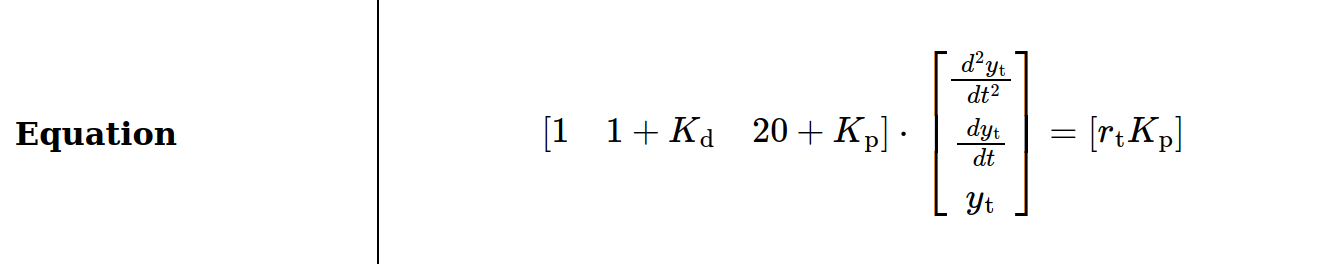
\includegraphics[width=1\textwidth]{figures/ODEInMatrix.png}
		\caption{Displaying ODE in a matrix form}
		\label{fig_multienv_odematrix}
	\end{subfigure}
	~
	\begin{subfigure}[t]{\textwidth}
		\centering
	
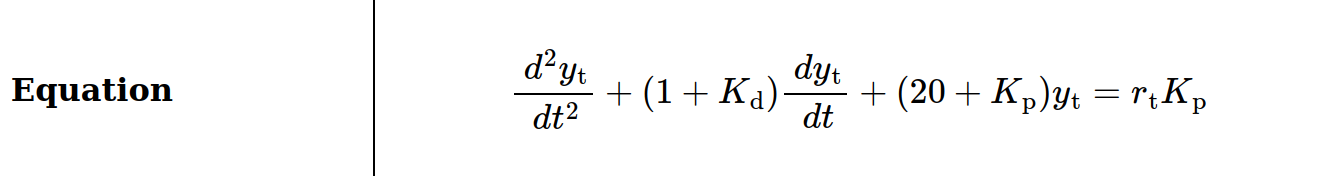
\includegraphics[width=1\textwidth]{figures/ODEInLinearEq.png}
		\caption{Displaying ODE in a linear equation}
		\label{fig_multienv_odelinear}
	\end{subfigure}
	
	\caption{Options of Displaying an ODE}
	\label{fig_multienv}
\end{figure}

1. We can display ODEs in a matrix form. The matrix form~\ref{eq_matrixformexmaple} is the prototype of how the ODE will appear in a matrix form in the SRS. In the \verb|DifferentialModel|, the \verb|_coefficients| is a list of lists \verb|Expr|, the unknown vector is a list of \verb|Unknown|, and the constant vector is a list of \verb|Expr|. It should be fairly straightforward for Drasil Printer to display them by printing each part sequentially. Figure~\ref{fig_multienv_odematrix} shows how to display a matrix of ODE in SRS. 

2. We also can display ODEs in a shape of a linear equation. Example~\ref{eq_odeexmaple} is the prototype of how the ODE will show up in the shape of a linear equation in the SRS. Displaying a single ODE in a linear equation is a special case. When there is only one single ODE, it would be over complicated to display it in a matrix form. We explicitly force Drasil Printer to display a single ODE in shape of a linear equation (Figure~\ref{fig_multienv_odelinear}).The example is just a demo shows Drasil Printer is capable to display an ODE in a matrix form (Figure~\ref{fig_multienv_odematrix}).

In the future, the Drasil team wants to explore more variability in representing ODEs. An ODE has various forms, and we want \verb|DifferentialModel| to represent as many forms as possible. One topic highlighted in the discussion is showing an ODE in a canonical form. However, many mathematicians have different opinions on a canonical form, and the name of canonical form has been used differently, such as normal form or standard form. More research on this part would help us better understand the knowledge of ODE.
